\chapter{Introduction}
\professor{Dr. Rashmi}
\professor{Ms. Aparna}
\professor{Mr. Amlendu Kumar}
\myskip

Optimising means the optimisation of certain things (functions): for example in business, to maximise the production or minimise the cost of production. We proceed with an example.

\begin{example}
	If there be a ship which is to be loaded with stocks of $N$ items (number of items being $x_i$), and weight of $i^{th}$ item be $w_i$, volume $v_i$, and value $p_i$ for $i = 1, 2, \ldots, N$. Cargo volume and weight are respectively $W$ and $V$. Then, the mathematical formulation can be thought of, as maximising
	$$\sum_{i=1}^N p_ix_i$$
	subject to the constraints
	$$\sum_{i=1}^N w_ix_i \le W, \quad \sum_{i=1}^N v_ix_i \le V,$$
	and each $x_i$ being necessarily non negative.
\end{example}

In each optimisation problems, such objectives are presented along with the related constraints.
Sometimes the constraints may be such that the feasible region between them is unfortunately empty. This case is called non-feasible case. Sometimes, the objective function line may coincide with some side of the feasible region; or in other event the objective line may as well never reach the feasible region at all. In the former case, there are infinite solutions, and in latter none.

\section{Graphical Solutions}

Graphical solutions help interpret and solve the systems with ease. However, they have their own (fair) share of drawbacks as well. Namely, that graphical methods are rendered useless in the case of functions in more variables than 2 variables. Then, the system can not be graphically represented. Then, other methods need be devised to relax the dependence on graphical methods.

\section{Simplex Method}

Consider a particular problem.

\begin{question}
	Maximise $z=4x_1 + 3x_2$ subject to the constraints $x_1 + x_2 \le 8, 2x_1 + x_2 \le 10$ and $x_1, x_2 \ge 0$.
\end{question}
\begin{solution}
	Here, we will change it into a standard form, such as to maximise
	$$z = 4x_1 + 3x_2 + 0x_3 + 0x_4$$
	subject to the constraints
	$x_1 + x_2 + x_3 = 8$, $2x_1 + x_2 + x_4 = 10$ and $x_1, x_2, x_3, x_4 \ge 0$ by making some substitutions. In general, this looks like maximising $z = c^Tx$ subject to $Ax=b$ and $x\ge 0$.
\end{solution}

We make some assumptions, namely that
$b \ge 0$, and that $\rank A = m (<n)$.
Now, the constraint $Ax=b$ can be changed into $B x_B = b$, which is called the basic solution.

\section{Transportation and Assignment Problems}

Transporation problems are a special kind of LPP's to transport a commodity from  a group of nodes, called sources to another
group of nodes, called destinations such that the
total cost of transporting the commodity is
minimized. We can mathematically denote it as minimising
	$$Z = \sum_{i = 1}^n \sum_{j = 1}^m x_{ij} c_{ij}$$
	subject to the constraints that $\sum_{j = 1}^n  x_{ij} = a_i$ and $\sum_{j = 1}^m x_{ij} = b_j$, where
	$x_{ij} \ge 0$ for all $i$ and $j$, $a_i$ is the quantity of commodity at origin $i$, $b_j$ is the quantity of commondity demanded at destination $j$, $c_{ij}$ is the cost of transportation from $i$ to $j$, and $x_{ij}$ is the quantity transported from $i$ to $j$.

\paragraph{}
Refer the presentation shared: {\ttfamily resources{\textbackslash}workshop day 1 session 2.pdf}, for a detailed example.

\chapter{Numerical Optimisation}
\professor{Dr. Brij Mohan}
\myskip

Numerical Optimisation is a field of applied Mathematics that focuses on finding the best solution to a problem from a set of possible solutions. It has a goal to minimise or maximise (or both simultaneously!) an objective function by adjusting the values of input variables within a specified range. 

Below we list the steps of optimisation.

\begin{enumerate}
	\item Problem formulation
	\item Function definition
	\item Constraints definition
	\item Feasible region definition
	\item {\itshape Initialisation}
	\item {\itshape Iteration}
	\item {\itshape Convergence}
\end{enumerate}

Now, we will deal with an example.

\begin{example}[Gradient Descent Method]
	This is an iterative optimisation technique that is used for finding the minimum of a function. The first step here is to find the initial parameter --- the initial numerical guess for the index. Then, compute the gradient and update your iterations. Let the objective function here be
	$$f(x) = ax^2 + bx + c.$$
	Then, the gradient here will be $\dd fx = 2ax + b$, and the updating rule then will be
	$$x_{\mathrm{new}} = x_{\mathrm{old}} - \mathrm{Learning\ rate} \times \left.\dd fx \right|_{x_{\mathrm{old.}}}$$
	Let's now consider $a = 1, b = -6, c = 9$ and the initial guess be $2$. Then, we can work with the following script of Mathematica software:
	
	\begin{lstlisting}[caption = {Mathematica code for Gradient Descent Method}, language = Mathematica]
		f[x_] := x^2 - 6x + 9;
		grad[x_] := f'[x];
		xold = 2;
		learningRate = 0.1;
		iterations = 10;
		For[i = 1, i <= iterations, i++,
			xnew = xold - learningRate * grad[xold];
			xold = xnew;
		]
		Print["Minimum value ", f[xnew], " achieved at x = ", xnew, "."]
	\end{lstlisting}
	
	\noindent
	The output of the above script will be as follows.
	
	\begin{lstoutput}
		Minimum value 0.0115292 achieved at x = 2.89263.
	\end{lstoutput}
	
	\noindent
	Increasing the learning rate will result in a faster convergence of $f(x)$ to zero.
	We note here that in optimisation, we are finding the value of $x$ such that the function is minimum. However, if we do the reverse process, {\itshape then} it will be a root finding problem.
\end{example}

\section{Root Finding Techniques}

There are numerous techniques to approximate roots for continuous polynomials. One being Bisection Method. In this method, we first find (or guess) a closed interval such that the values of the function at the extreme points of this interval. If the interval is $[a, b]$, then we shall necessarily have $f(a)f(b) < 0$. Here, the initialisation is to set a mid point of the interval so that this interval divides the original interval into two closed intervals. We now apply the same idea to both these intervals and determine which interval contains the root {\itshape now}\footnote{It is interesting to note that both intervals may as well contain a root too!}.

\begin{algorithm}
	\caption{Algorithm for Bisection Method: $n$ iterations}
	\begin{algorithmic}
		\State $i \gets 0$
		\While{$i < n$}
		\State $c \gets \frac{a + b}2$
		\If{$\sign{f(b)} = \sign{f(c)}$}
		\State $b \gets c$
		\Else
		\State $a \gets c$
		\EndIf
		\EndWhile
	\end{algorithmic}
\end{algorithm}

\section{Secant Method}
Another method is the Secant Method. We saw that the changes being made in Bisection Method was linear. We remember the rate of convergence and order of convergence here. Walk 5 meteres, and run 5 meters: the time and steps taken to do such travel changes in each case. The degree of optimality is the order of convergence, while the ratios between errors in each iteration is rate.

In this method, we initialise the interval, and the iterative function for indices is given by
$$p_{n + 1} = p_n - f(p_n) \frac{p_n - p_{n -1}}{f(p_n) - f(p_{n - 1})}.$$
Convergence holds here, and this can be seen algebraically by paying attention to $f_{n} - p$ at $n^{\mathrm{th}}$ iteration.

\section{Newton's Method}
Newton's Method is similar. He changed the iterative formula to
$$p_{n + 1} = p_n - \frac{f(p_n)}{f'(p_n)}.$$
The efficiency here, however, is different. This method comes with a convergence rate of $2$ --- highest in all, \emph{yet}. The following Mathematica Code will approximate zeroes of a polynomial.

\begin{lstlisting}[caption = {Mathematica Script for Newton's Root Finding Method}, language = Mathematica]
	newtonMethod[expr_, var_, l_List, n_ : 10, eps_ : 0.0000005] := Module[
		{f, fv, xc,  init, deriv},
		Catch[
			init = (l[[1]] + l[[2]])/2;
			f[fv_] := expr /. var -> fv;
			deriv = f'[var];
			For[i = 1, i <= n, i++,
			xc = init - f[init]/(deriv /. var -> init);
			If[Abs[f[xc]] <= eps, Throw[{i, N[xc, 10], N[f[xc], 10]}]];
			init = xc
			];
			Throw[{n, N[xc, 10], N[f[xc], 10]}]
		]
	]
\end{lstlisting}


\paragraph{Iterative Techniques}
In this section, we will discuss about some iterative techniques to solve numerical optimisation problems surrounding matrices.

\section{Gauss-Jacobi Method}
We will talk about the Jacobi Method first of all. We initialise the matrix
$$X^{(0)} = \begin{bmatrix}
	x_1^{(0)} & x_2^{(0)} & \ldots & x_n^{(0)}
\end{bmatrix}$$
and the iteration is then
$$x_i^{(k+1)} = \frac{1}{a_{ii}} \left[ b_i - \sum_{j=1; \, j \not= i}^n a_{ij}x_j^{(k)}\right].$$
Convergence holds as $\| X^{(k+1)} - X^{(k)} \| < \epsilon.$

\begin{lstlisting}[caption = {Gauss-Jacobi Method in Mathematica}]
	gJMethod[A_List, maxiters_ : 10] := Module[
		{n, tuple},
		n = Dimensions[A][[1]];
		Catch[
			If[Dimensions[A][[1]] + 1 == Dimensions[A][[2]], Nothing[], Throw["Invalid matrix supplied."]];
			tuple = Table[0, {i, n}];
			For[i = 1, i <= maxiters, i++,
				For[ni = 1, ni <= n, ni++, 
					tuple[[ni]] = N[1/A[[ni]][[ni]] (A[[ni, n + 1]] - Sum[A[[ni, r]] tuple[[r]], {r, Complement[Table[1, n], {ni}]}]), 10];
				];
			];
			Throw[{i - 1, tuple}]
		]
	]
\end{lstlisting}

\section{Gauss-Seidal Method}
Then, the Gauss-Seidal Method comes, which is an instance of Gauus-Jacobi however with relative weighting. The iteration here is 
$$x_i^{(k+1)} = (1-w)x_i^{(k)} + \frac{w}{a_{ii}} \left[ b_i - \sum_{j=1; \, j \not= i}^n a_{ij}x_j^{(k)}\right]$$
where $w$ is the implied weight.

\chapter{Logistic Regression In ML}
\professor{Prof. Amber}
\professor{Prof. Prashant}
\myskip


Assume we have a set of data point $\{x_i\in \bb R^d\}$, with each $x_i$ having exactly one label, say $y_i = 1$ or $y_i = 0$. Then, 
$$\{(x_1, y_1), (x_2, y_2), \ldots, (x_N, y_N)\}$$
are the data points we have, each $y_i$ belonging to $\{0, 1\}$. Now, if we have another data point, say $x$, can we extract some information from the existing data set to identify whether $x$ belongs to category (label) zero, or one? We here introduce a function
$$p(y = 1 | x) = \frac{1}{1 + e^{-\theta^{\mathrm T}x}}; \quad p(y = 0|x) = 1 - p(y = 1|x) = \frac{e^{-\theta^{\mathrm T}x}}{1 + e^{-\theta^{\mathrm T}x}}.$$
What we want here is to determine $\theta$ --- a parameter, such that it correctly predicts the categories of the known dataset.

\paragraph{}
Let
$$C(i) = - \left[y_i \log\pi(i) + (1-y_i) \log\big(1-\pi(i)\big)\right],$$
where $\pi(i) = \frac{1}{1 + e^{-\theta^{\mathrm T}x}}$, be the cost of predicting $x_i$ correctly. Let us say that $x_i \in y_i = 1$ and $\theta$ is such that $\pi(i) = 1$. Then here, the cost of predicting also comes out to be zero. This function is called {\itshape cost-entropy based function}. Now, let
$$C(\theta) = -\sum_{i = 1}^N \left[y_i \log\pi(i) + (1-y_i) \log\big(1-\pi(i)\big)\right]$$
be the cost prediction function for all $N$ data-points, withstanding the same definition of $\pi$ as before.

\paragraph{Our Problem}
We now wish to find $\min_{\theta \in \bb R^d} C(\theta)$. 

\begin{example}
	Let $f(x) = x^2 + 2x+1$. To minimise this, we find the critical points and try to find the extrema points. Now, consider that
	$$\nabla_\theta C(\theta) = \begin{bmatrix} \dd{C(\theta)}{\theta_1} & \dd{C(\theta)}{\theta_2} & \dots & \dd{C(\theta)}{\theta_d} \end{bmatrix}.$$
	And, $\nabla_\theta^2$ will belong to $\bb R^{d \times d}$ and the $(i,j)^{\mathrm{th}}$ component will be nothing but $\frac{\partial^2 C(\theta)}{\partial\theta_i\partial\theta_j}$, with eigen values being non-negative.
\end{example}

\section{Iterative Descent Idea}
Minimising the above friend is a tiresome process. Therefore comes iterative methods to ease the process.

$$\theta_{k+1} = \theta_k + \alpha_k d_k$$
where the $\theta_k$ is step size, $d_k$ the descent direction, and $\alpha_k$ a positive number. Here, we start with an initial condition, say $\theta_0$ and progress such as
$$\theta_0 \to \theta_1 \to \theta_2 \to \dots \mathrm{as}\ k \to \infty.$$
We assume that $d_k$ is the gradient of $C$ at $\theta_k$, that is, $d_k = -\nabla C(\theta_k) \in \bb R^d$.
\marginnote{If $\alpha_k$ is such that, at every iteration, $C(\theta_{k+1}) \le C(\theta_k)$, then eventually as $k\to\infty$, we find a [local] minimum.}
Consider
\begin{align*}
	C(\theta_{k+1}) &= C\big(\theta_k - \alpha_k \nabla C(\theta_k)\big) \\
	&=C(\theta_k) - \alpha_k\left( \nabla C(\theta_k) \right)^{\mathrm{T}}\left(\nabla C(\theta_k)\right) + O(\alpha_k).
\end{align*}
We will make an assumption here that $\alpha_k\to0$, and under this assumption, we overrule this term from the above expression, replacing equality with approximity. Note that
$$\alpha_k\left( \nabla C(\theta_k) \right)^{\mathrm{T}}\left(\nabla C(\theta_k)\right)$$
will be a non-negative quantity, and so we can guarantarily derive that $C(\theta_{k+1}) \le C(\theta_k)$ if we use this algorithm with sufficiently small $\alpha_k$. Essentially, we are decreasing the value of cost at every iteration of the gradient descent, and eventually, we will reach the desired minimum.

\paragraph{}
As for the value of $\alpha$, one of the ways to find it is hit and trial. But there are more prudent ways to get that value. $\alpha_k = \frac1k$ is another way that is dependent on $k$, rather than a hit and trial method. As $k$ becomes large, $\alpha_k$ is going to zero. Or, we can assume that the gradient of the cost function Lipschitz, that is
$$\|\nabla C(\theta) - \nabla C(\phi) \| \le L \| \theta - \phi \|,$$
then choosing $\alpha$ in $\left(0, \frac2{L}\right)$ will guarantee the reach to minimum.

\section{Linear Regression}

Linear Regression is one of the simplest prediction 
\marginnote{predictions --- future guesses for something that we do not know using current data-sets.}
techniques. We here deal with an example.

\begin{example}
	The state government wishes to build a lot of buildings. They wish to decide the price tag for each building. They may refer the data-sets for previous instances and look for factors including number of rooms, or vicinity of train stations, availability of lifts, and others.
	
	\paragraph{}
	The problem here is to find (predict) the price of a house/apartment/flat given the past data. This past data includes
	\begin{enumerate}
		\item the set of factors influencing price of the house: causality  between a building having a lift and the settlement of the price, for example; and
		\item a label (or, a price) corresponding to each data point.
	\end{enumerate}
	
	We hypothesis here that all of these factors affect the price in a linear (though unknown) fashion. Let us assume that this relation is given by
	$$\hat y = \theta_0 + \sum_{i=1}^n \theta_i \hat x_i.$$
	Now, the error will be
	$$\sqrt{\sum_{j=1}^m \left[ \hat y^j - \left(\theta_0 + \sum_{i=1}^n \theta_i \hat x_i^j\right)\right]^2}.$$
	
	\paragraph{Optimisation Problem}
	We need to minimise here the above error term. That is, the $\theta_i$'s are needed to be found, that are bound to no constraints. Define
	$$Y = \begin{bmatrix} \hat y_1 & \hat y_2 & \dots & \hat y_m \end{bmatrix},$$
	and $X$ be the $(m+1)\times n$ matrix. Then, the error function will be given by
	$$\min_\theta (Y - X\theta)^{\mathrm T} (Y - X\theta).$$
	We find now the derivative and set it zero to obtain
	$$-X^{\mathrm T}Y + 2X^{\mathrm T}X\theta - (Y^{\mathrm T}X)^{\mathrm T} = 0$$
	implying further than $\theta = (X^{\mathrm T}X)\inv X^{\mathrm T} Y.$
	This requires heavy computations, hence we resort to Gradient Descent Method. Begin with $\vec\theta^0$ and update $\vec\theta^1 = \vec\theta^0 + \alpha (-\nabla f)$, continuing until we can sustainably stop. This stopping criterion could be, namely that $|\theta^{k+1} - \theta^k|$ shall be very small.
\end{example}

\chapter{Machine Learning}
\professor{Prof. Suresh Chandra}
\myskip

Machine Learning is the development of algorithms trained by data-sets. To understand this, we proceed with an example.

\begin{example}
	Consider loan giving facility in a bank. The bank has certain datasets including, say $k$ points of the form $(x_i, y_i)$ where $x_i$ is in $\bb R^n$ containing information about the respective loan request. $y_i$ be the label --- $1$ if the loan was given, $-1$ if not; then this data-set can be used to derive whether another point, say $x$, be labelled $1$ or $-1$.
	
	\begin{figure}[h]
		\centering
		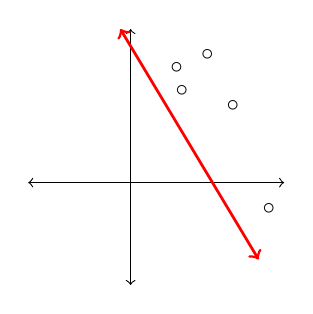
\begin{tikzpicture}[scale = 0.65]
			\draw[<->] (-2, 0) -- (3, 0);
			\draw[<->] (0, -2) -- (0, 3);
			\node[label = \scalebox{.5}{$\square$}] at (0, 0.1) {};
			\node[label = \scalebox{.5}{$\square$}] at (-.5, 2) {};
			\node[label = \scalebox{.5}{$\square$}] at (1.2, -1) {};
			\node[label = \scalebox{.5}{$\square$}] at (.7, -1.2) {};
			\node[label = \scalebox{.5}{$\square$}] at (-1, 1) {};
			\node[label = \scalebox{.5}{$\square$}] at (-1.3, 1.3) {};
			
			\node[label = \scalebox{.9}{$\circ$}] at (2, 1) {};
			\node[label = \scalebox{.9}{$\circ$}] at (1, 1.3) {};
			\node[label = \scalebox{.9}{$\circ$}] at (0.9, 1.75) {};
			\node[label = \scalebox{.9}{$\circ$}] at (1.5, 2) {};
			\node[label = \scalebox{.9}{$\circ$}] at (2.7, -1) {};
			
			\draw[<->, red, line width = 1pt] (-0.2, 3) -- (2.5, -1.5);
		\end{tikzpicture}
	\end{figure}
	
	It can be thought of as shown in the figure above. The points to the left of the red line (squares) be the positive ones, and those to the right (circles) be the negative ones. Then, the red line in figure is called the separator. In this case, this separator is linear. Then, similarly, the labels of newer points can be determined by their positioning relative to the red line. The fitting of this red line is done by using already existing data-sets.
\end{example}


\section{Well or Ill}

\newcommand\tikzcheck{{\color{green}\textcircled{\checkmark}}}
\begin{center}
	\begin{tikzpicture}
		\node[black, line width = 2pt] at (0, 0) (problems) {{\Large\bfseries Problems}};
		\node[below left = 2cm of problems, yshift = .35cm] (direct) {{\large\bfseries Direct}};
		\node[below right = 2cm of problems, yshift = -.5cm] (indirect) {{\large\bfseries Indirect}};
		\path[black, out = 240, in = 70, ->] (problems) edge (direct);
		\path[black, out = 300, in = 110, ->] (problems) edge (indirect);
		
		\node[below = .125cm of direct, black, line width = .4pt, draw, inner sep = .3cm] (inf) {Function $f$ \tikzcheck};
		\node[left = 1.25cm of inf] (infl) {};
		\node[right = 1.25cm of inf] (infr) {};
		\draw[->] (infl) -- (inf);
		\draw[->] (inf) -- (infr);
		\node[left = 0cm of inf, yshift = .25cm, ] {input \tikzcheck};
		\node[left = .5cm of inf, yshift = -.25cm] {$x$};
		
		\node[left = 1.25cm of inf] (infl) {};
		\node[right = 1.25cm of inf] (infr) {};
		\draw[->] (infl) -- (inf);
		\draw[->] (inf) -- (infr);
		\node[right = .1cm of inf, yshift = .25cm, ] {output};
		\node[right = .3cm of inf, yshift = -.25cm] {$f(x)$};
		\node[right = 0cm of infr, red] {\textcircled{\raisebox{-1pt}{\scalebox{.8}{?}}}};
		\node[below = .25cm of inf, draw, rounded corners] {Well-posed function};
		
		\node[below = .125cm of indirect, black, line width = .4pt, draw, inner sep = .3cm] (ouf) {Function $f$ {\color{red}\textcircled{\raisebox{-1pt}{\scalebox{.8}{?}}}}};
		\node[left = .25cm of ouf] {${x^{(i)}}_{i=1}^p$ \tikzcheck};
		\node[right = .25cm of ouf] {${y^{(i)}}_{i=1}^p$ \tikzcheck};
		\node[below = .25cm of ouf, draw, rounded corners] {Ill-posed function};
	\end{tikzpicture}
\end{center}

\noindent
Consider the example shown below.

\begin{figure}[h]
	\centering
	\begin{tikzpicture}
		\draw[<->] (-0.5, 0) -- (1.5, 0);
		\draw[<->] (0, -0.5) -- (0, 1.5);
		\node[label = \scalebox{.5}{$\square$}] at (0, 0) {};
		\node[label = \scalebox{.5}{$\square$}] at (1, 0) {};
		\node[label = \scalebox{.5}{$\square$}] at (0, 1) {};
		\node[label = \scalebox{.8}{$\circ$}] at (1, 1) {};
	\end{tikzpicture}
\end{figure}

\noindent
Then, here the sets $A$ and $B$ will be
$$A = \begin{bmatrix}
	0 & 0 \\ 1 & 0 \\ 0 & 1
\end{bmatrix}, \quad \mathrm{and,} \quad
B = \begin{bmatrix}
	1 & 1
\end{bmatrix}.$$


\section{Linear Separability}
Convex set is a set containing all of the points in the given data-set, while convex hull is the {\itshape smallest} such set.
Two sets are said to be linearly separable if their {\itshape convex hulls} are disjoint. Existence of a plane which strictly separates the sets is guaranteed by the Strict Separation Theorem. However, linear separability holds if and only if this plane is linear. If there does not exist such a plane (and in that case a curve exists), then the separability is non-linear. In our problem, if $w\trans x = b$ is the plane, then the points having label $+1$ will satisfy $w\trans > b$ and those having label $-1$ will do $w\trans < b$. More formally, the problem is to solve
$$\left\{\begin{matrix}
	Aw > be, \\ Bw < be, \\ w \in \bb R^n, b \in \bb R,
\end{matrix}\right.$$
which can be equivalently expressed as
$$\left\{\begin{matrix}
	Aw > eb \le e, \quad \forall y_1 = 1, \\ Bw + be \le e, \quad \forall y_i = -1, \\ w \in \bb R^n, b \in \bb R,
\end{matrix}\right.$$

\section{Measuring Error of Misclassification}

$$\boxed{\frac1m\left\|(-Aw + eb + e)_+ \right\|_1 + \frac1k \left\| (Bw -eb  + e)_+ \right\|_1.}$$
Our aim here is to minimise the above average infeasibilities. Here, $(X_+)_i = \max(X_i, 0)$ and $\|X\|_1$ is the norm $\sum_{i=1}^l|S+i|$.

\begin{question}
	Let
	$$S = \begin{bmatrix}
		1 & 1
	\end{bmatrix}, \quad \mathrm{and,} \quad
	B = \begin{bmatrix}
		0 & 0 \\ 1 & 0 \\ 0 & 1
	\end{bmatrix}.$$
	Solve.
\end{question}
\begin{solution}
	The LPP formulation for this problem is to minimise $y = \frac13(z_1+z_2+z_3)$ subject to the constraints
	\begin{align*}
		w_1+w_2-b+y \ge 1, \\
		b+z_1 \ge 1, \\
		-w_2 + b + z_2 \ge 1, \\
		-w_2 + b + z_3 \ge 1, \\
		y,z_1,z_2,z_3 \ge 0,
	\end{align*}
	with $w_1,w_2, b$ being unrestricted. The solution to this LPP is $(w_1,w_2,b)=(2,2,3)$, hence the equation of the separating plane is $x_1+x_2 = 1.5$.
\end{solution}

\begin{example}[XOR Problem: Linearly Inseparable]
	Consider 
	$$A = \begin{bmatrix}1&0\\0&1\end{bmatrix}, \quad \mathrm{and,}\quad
	B = \begin{bmatrix}0&0\\1&1\end{bmatrix}.$$
	Then, we will have $\frac{eA}{2} = \frac{eB}{2}$. Therefore, $w=0, b=0, y=e, z=e$ is a solution. 
\end{example}